\documentclass[12pt]{article}
\usepackage[english]{babel}
\usepackage{natbib}
\usepackage{url}
\usepackage[utf8x]{inputenc}
\usepackage{amsmath}
\usepackage{graphicx}
\usepackage{float}
\usepackage{hyperref}
\graphicspath{{images/}}
\usepackage{parskip}
\usepackage{fancyhdr}
\usepackage{listings}
\usepackage{hyperref}
\usepackage{color}
\usepackage{float}

\definecolor{codegreen}{rgb}{0,0.6,0}
\definecolor{codegray}{rgb}{0.5,0.5,0.5}
\definecolor{codepurple}{rgb}{0.58,0,0.82}
\definecolor{backcolour}{rgb}{0.95,0.95,0.92}

\makeatletter
\let\oldfigure\figure
\let\endoldfigure\endfigure
\renewenvironment{figure}[1][]{\oldfigure[H]}{\endoldfigure}
\makeatother

\lstdefinestyle{mystyle}{
    backgroundcolor=\color{backcolour},   
    commentstyle=\color{codegreen},
    keywordstyle=\color{magenta},
    numberstyle=\tiny\color{codegray},
    stringstyle=\color{codepurple},
    basicstyle=\ttfamily\footnotesize,
    breakatwhitespace=false,         
    breaklines=true,                 
    captionpos=b,                    
    keepspaces=true,                 
    numbers=left,                    
    numbersep=5pt,                  
    showspaces=false,                
    showstringspaces=false,
    showtabs=false,                  
    tabsize=2
}

\lstset{style=mystyle}
\renewcommand{\lstlistingname}{Snippet}
\renewcommand{\lstlistlistingname}{Snippets}
\def\lstlistingautorefname{Snippet}



\hypersetup{
    colorlinks=true,    % Enable colored links instead of boxed links
    linkcolor=black,     % Color for internal links (sections, pages)
    urlcolor=black,      % Color for external URLs
    citecolor=black,     % Color for citation links
    filecolor=black   % Color for file links
}
%\usepackage{vmargin}
%\setmarginsrb{2 cm}{2.5 cm}{3 cm}{2.5 cm}{1 cm}{1.5 cm}{1 cm}{1.5 cm}

\topmargin=-0.2in    
\textheight=9in     %24.1cm
\evensidemargin=0in %0cm
\oddsidemargin=0in  %-.3cm
\textwidth=6.5in    %16.5cm

\title{Assignment Name \\ about \\ \vspace{0.5cm} Subject}								% Title
\author{Yassien E4}								% Author
\date{\today}											% Date

\makeatletter
\let\thetitle\@title
\let\theauthor\@author
\let\thedate\@date
\makeatother

\pagestyle{fancy}
\fancyhf{}
\rhead{\theauthor}
\lhead{School of Computing}
\rfoot{\thepage}

\begin{document}
\vspace{-2cm}
%%%%%%%%%%%%%%%%%%%%%%%%%%%%%%%%%%%%%%%%%%%%%%%%%%%%%%%%%%%%%%%%%%%%%%%%%%%%%%%%%%%%%%%%%

\begin{titlepage}
	\centering
    %\vspace*{0.1 cm}
    \includegraphics[scale = 1]{logo.png}\\[1.0 cm]	% University Logo
    \textsc{\LARGE The Knowledge Hub \\ \vspace{0.5cm} Universities}\\[1.5 cm]	% University Name
	\textsc{\Large KH00000XXX}\\[0.5 cm]				% Course Code
	\textsc{\large Module Name}\\[0.5 cm]				% Course Name
	\rule{\linewidth}{0.2 mm} \\[0.4 cm]
	{ \huge \bfseries \thetitle}\\
	\rule{\linewidth}{0.2 mm} \\[1.5 cm]
	
    {\large \thedate}\\[1 cm]
    
	\begin{minipage}{0.4\textwidth}
		\begin{flushleft} \large
			\emph{Author:}\\
			\theauthor
			\end{flushleft}
			\end{minipage}~
			\begin{minipage}{0.4\textwidth}
			\begin{flushright} \large
			\emph{Student ID:} \\
			CU0000000									% Your Student Number
		\end{flushright}
	\end{minipage}\\
	
	
 
	\vfill
	
\end{titlepage}

%%%%%%%%%%%%%%%%%%%%%%%%%%%%%%%%%%%%%%%%%%%%%%%%%%%%%%%%%%%%%%%%%%%%%%%%%%%%%%%%%%%%%%%%%
\pagenumbering{gobble}
\tableofcontents
\pagebreak

\raggedbottom


% IF YOU WANT A LIST OF TABLE AND LIST OF FIGURES UNCOMMENT THE LINES DOWN HERE
% \pagenumbering{gobble}
% \listoffigures
% \listoftables
% \newpage


%%%%%%%%%%%%%%%%%%%%%%%%%%%%%%%%%%%%%%%%%%%%%%%%%%%%%%%%%%%%%%%%%%%%%%%%%%%%%%%%%%%%%%%%%
\pagenumbering{arabic}
\section{Task 1: Shell}
\href{https://github.com/yassienE4/OS-VM/commit/929f4ec3803c7845995459e7b9b7fca693f79cf8}{\ul{https://github.com/yassienE4/OS-VM/commit/929f4ec3803c7845995459e7b9b7fca693f79cf8}}

\subsection*{How to Run}
\begin{enumerate}
\item cd The-Shell
\item ./run.sh main.cpp
\item If running in file mode, compile with g++ -std=c++17 -w main.cpp -o main and run ./main args
\end{enumerate}

The code accepts a text file as input and reads commands from it line by line. If no arguments are provided, it starts an interactive loop instead.

\begin{figure}[H]
\centering
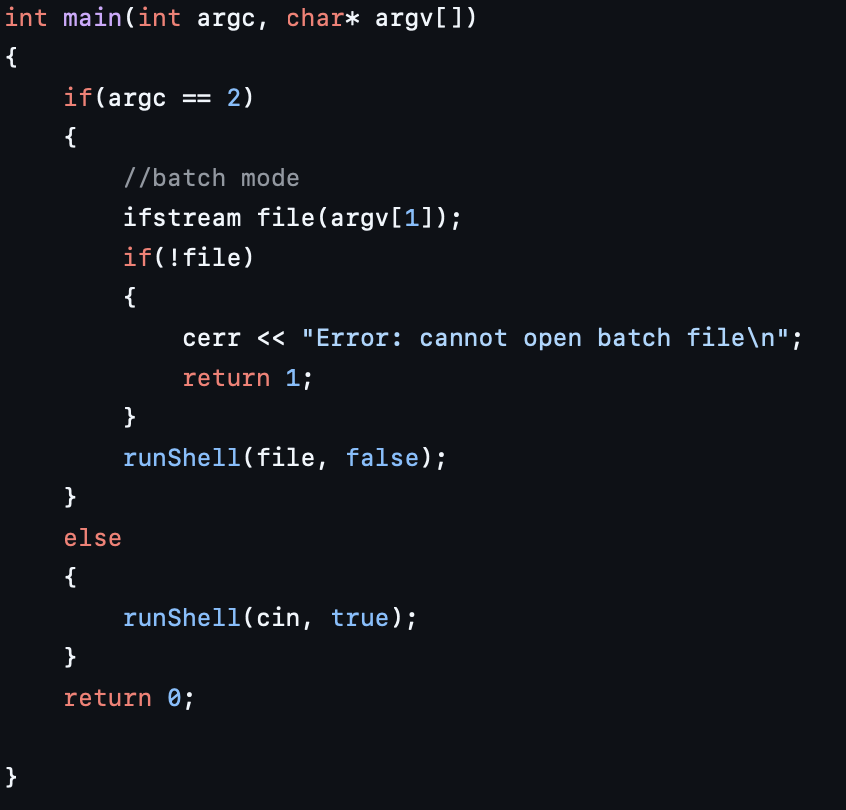
\includegraphics[width=4.8in]{./images/report1/image2.png}
\caption{Interactive command input}
\end{figure}


The commands are parsed into a custom data structure in \texttt{commands.h} with the following fields:

\begin{itemize}
\item name
\item args
\item inFile
\item outFile
\item append
\item background
\item isBuildIn
\end{itemize}

\begin{figure}[H]
\centering
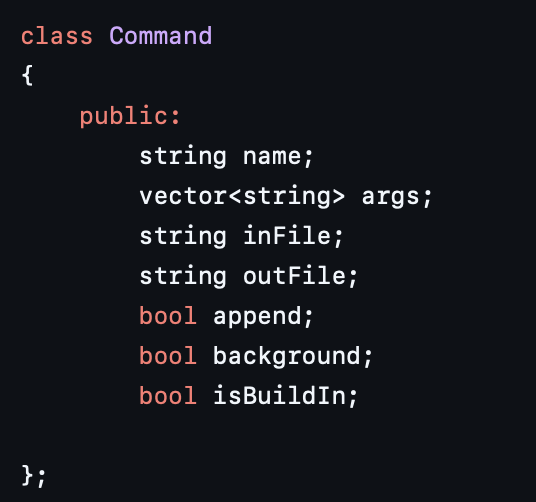
\includegraphics[width=4.8in]{./images/report1/image1.png}
\caption{Command data structure}
\end{figure}


The structure makes it possible to determine how each command should be handled, including whether it is a built-in command, whether it should run in the background, and whether it reads from or writes to a file. Commands are then executed either through forking and process execution or through C system functions for built-in behavior.

\begin{figure}[H]
\centering
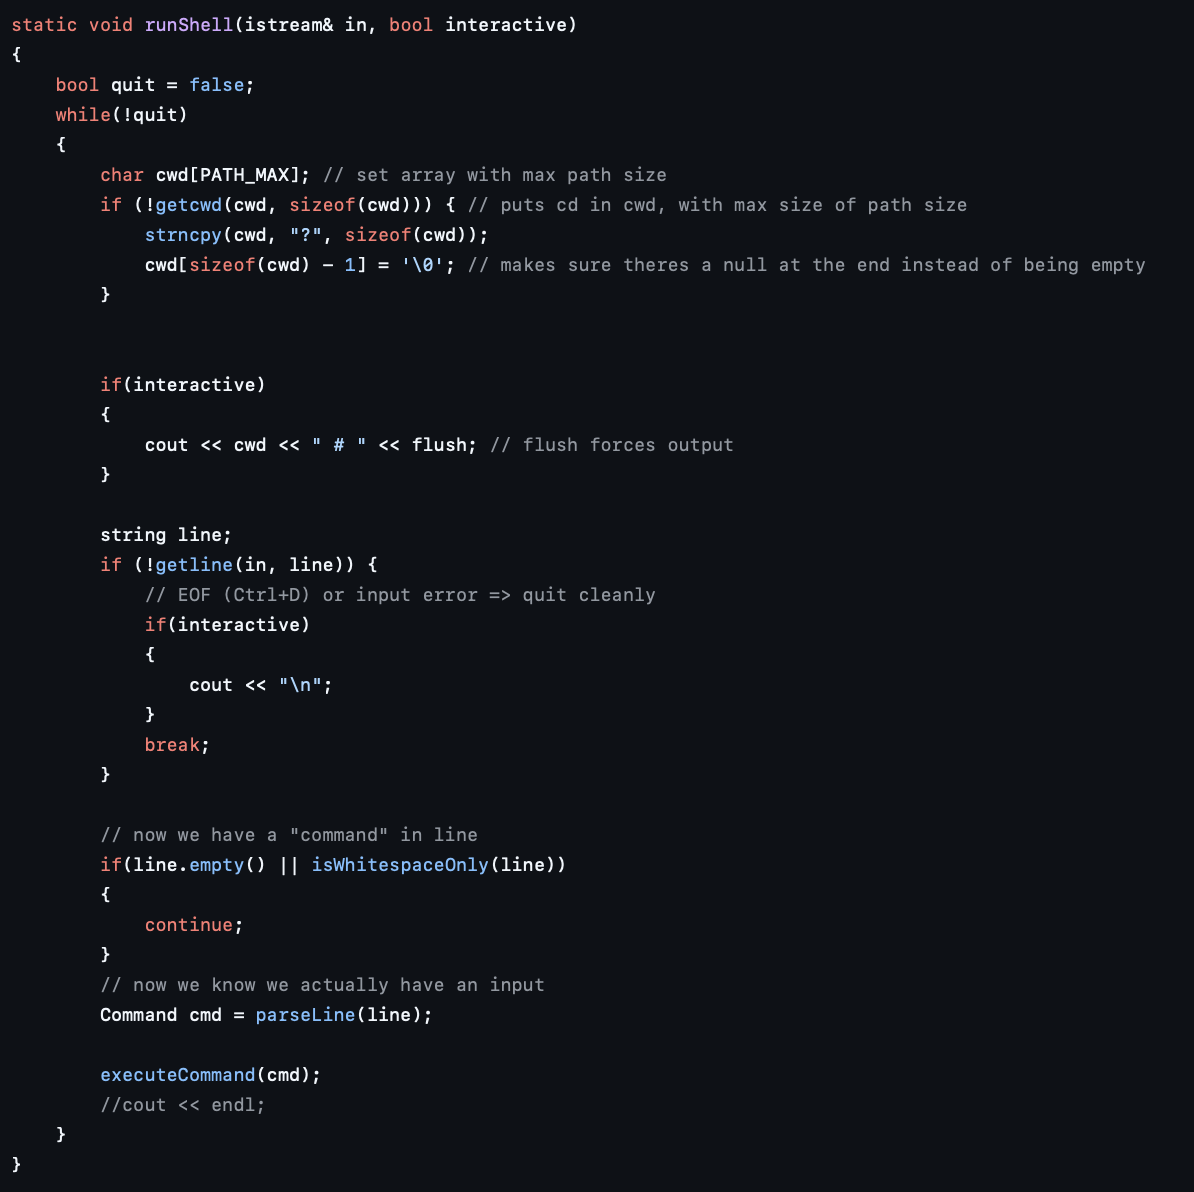
\includegraphics[width=6.5in]{./images/report1/image3.png}
\caption{Command execution flow}
\end{figure}

\begin{figure}[H]
\centering
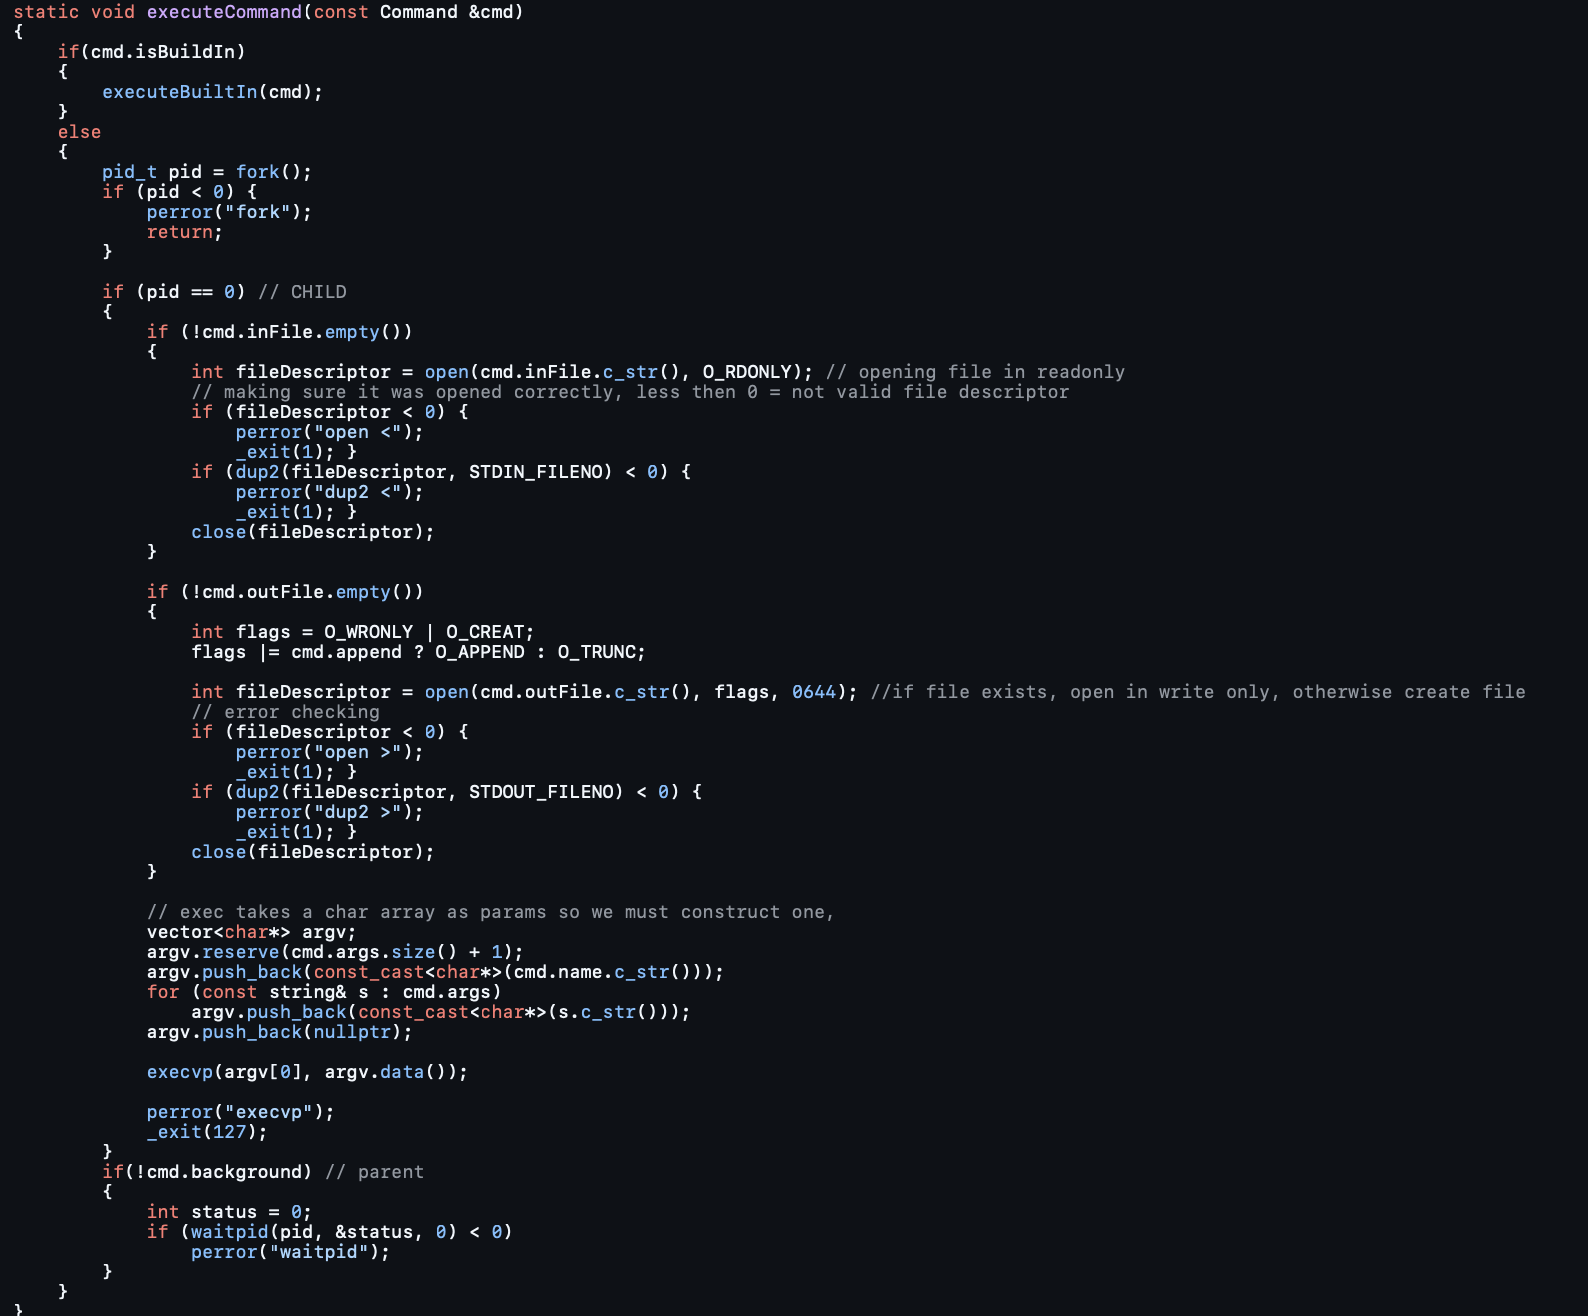
\includegraphics[width=6.5in]{./images/report1/image4.png}
\caption{Built-in command handling}
\end{figure}

\begin{figure}[H]
\centering
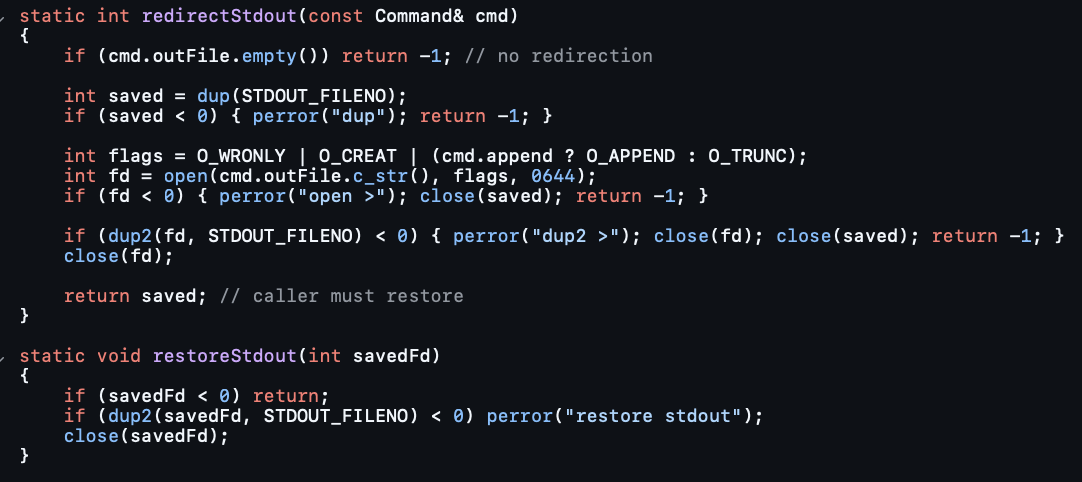
\includegraphics[width=5.8in]{./images/report1/image5.png}
\caption{Command parsing detail}
\end{figure}

\begin{figure}[H]
\centering
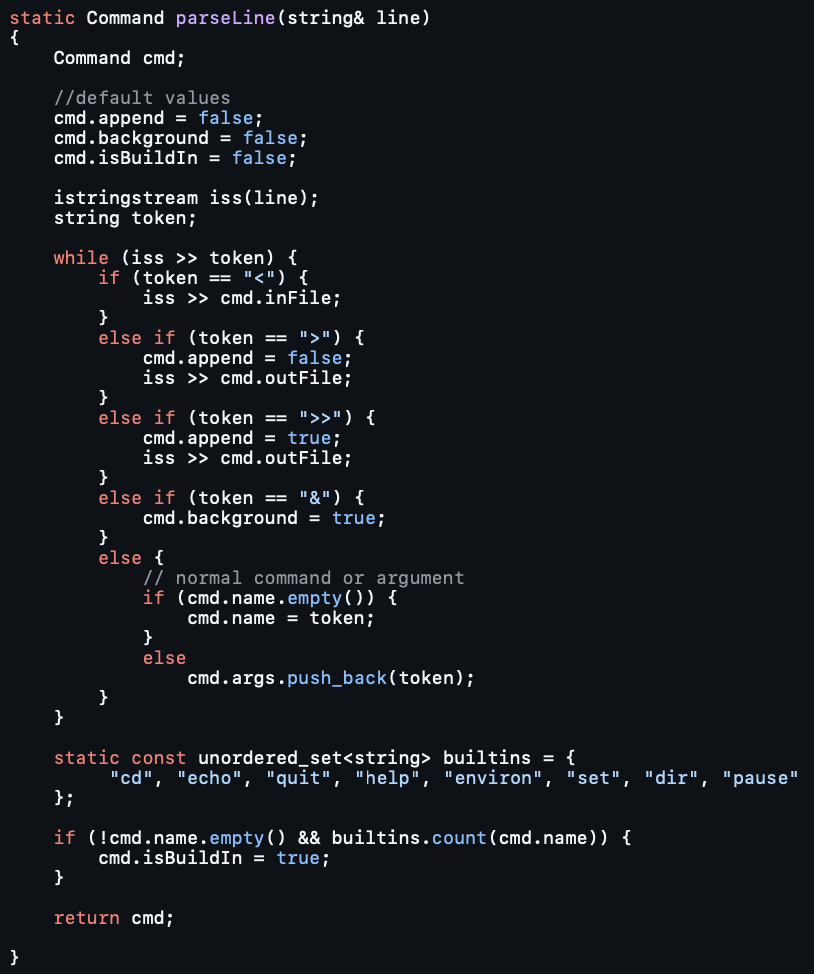
\includegraphics[width=5.8in]{./images/report1/image6.png}
\caption{Background execution handling}
\end{figure}

\begin{figure}[H]
\centering
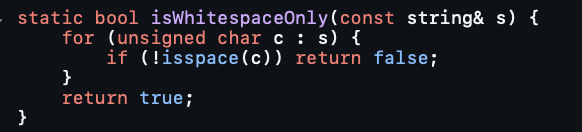
\includegraphics[width=3.8in]{./images/report1/image7.png}
\caption{File redirection handling}
\end{figure}

\section{Task 2: Multithreaded Word Count}
\href{https://github.com/yassienE4/OS-VM/commit/48d51e62658d47fa3c8d2de21cb3f8fb4115c635}{\ul{https://github.com/yassienE4/OS-VM/commit/48d51e62658d47fa3c8d2de21cb3f8fb4115c635}}

\subsection*{How to Run}
\begin{enumerate}
\item cd task2
\item ./run.sh main.cpp
\item ./main \textless text path \textgreater{} \textless number of threads used \textgreater{}
\end{enumerate}


The program takes two parameters: a text file and the number of threads to use. The provided \texttt{test.txt} file can be used as an example input.

\begin{figure}[H]
\centering

\includegraphics[width=4.8in]{./images/report2/image1.png}
\caption{Word count overview}
\end{figure}

\begin{figure}[H]
\centering

\includegraphics[width=6.2in]{./images/report2/image4.png}
\caption{Thread segmentation and map setup}
\end{figure}

\begin{figure}[H]
\centering

\includegraphics[width=5.5in]{./images/report2/image5.png}
\caption{Thread processing view}
\end{figure}

The text is split into \(n\) roughly equal segments without cutting words in half. To do that, the code checks the chunk boundary and advances until it reaches a non-alphanumeric character. This produces pairs of start and end indices for each segment.

Once the text is split, the program creates one thread per segment and lets each thread count words into a local map. After all threads finish, the local maps are merged into a final map containing the total occurrence count for each word.

\begin{figure}[H]
\centering

\includegraphics[width=5.8in]{./images/report2/image2.png}
\caption{Local map consolidation}
\end{figure}

\begin{figure}[H]
\centering

\includegraphics[width=5.5in]{./images/report2/image6.png}
\caption{Final word count output}
\end{figure}

\section{Task 3: Aging Page Replacement}
Theory:

We want to map processes, or pages, to physical memory frames. When there are no more frames, we need to know which page to replace. The aging algorithm picks the least recently used page.

\subsection*{How to Run}
\begin{enumerate}
\item cd paging
\item ./run.sh main.cpp
\item ./main \textless text path \textgreater{} \textless max frames \textgreater{}
\end{enumerate}

The code first parses a text file into a vector using \texttt{readReferences()}. For example, \texttt{TXT [0 1 2 3]} becomes \(\{0,1,2,3\}\).

\begin{figure}[H]
\centering

\includegraphics[width=5.2in]{./images/report3/image1.png}
\caption{Reference parsing output}
\end{figure}

\begin{figure}[H]
\centering

\includegraphics[width=5.8in]{./images/report3/image2.png}
\caption{Aging algorithm overview}
\end{figure}

The simulation then runs the aging algorithm for every frame count from 1 up to the maximum. Each frame stores:

\begin{itemize}
\item page
\item counter
\item referenced flag
\end{itemize}

\begin{figure}[H]
\centering

\includegraphics[width=3.8in]{./images/report3/image4.png}
\caption{Frame state during simulation}
\end{figure}


For each reference, the program shifts every frame counter, marks recently used frames, checks whether the page is already loaded, and loads it if necessary. If there is an empty frame, the page is inserted directly. If memory is full, the frame with the lowest counter is replaced under the assumption that the smallest counter corresponds to the least recently used page.

\begin{figure}[H]
\centering

\includegraphics[width=4.6in]{./images/report3/image5.png}
\caption{Page replacement decision}
\end{figure}


After the simulation, the program calculates \((faults \times 1000.0) / references.size()\) and stores the result in a CSV file.

\subsection*{Testing}
I found that after the number of unique pages, the number of maximum frames no longer matters. For example, if the pages are 0 through 10, then there are 11 unique pages, and after 11 frames the frame count does not change the number of faults. The only remaining faults are the initial faults from loading each unique page.

\begin{figure}[H]
\centering

\includegraphics[width=3.8in]{./images/report3/image6.png}
\caption{Page fault results}
\end{figure}

\begin{figure}[H]
\centering

\includegraphics[width=6.4in]{./images/report3/image7.png}
\caption{Testing observations}
\end{figure}


\section{Task 4: Deadlock Detection}
\href{https://github.com/yassienE4/OS-VM/commit/3846ae8b48fa572486c9cc3fb142f36fbf4de522}{\ul{https://github.com/yassienE4/OS-VM/commit/3846ae8b48fa572486c9cc3fb142f36fbf4de522}}

\subsection*{How to Run}
\begin{enumerate}
\item cd deadlock
\item Change \texttt{input.txt} to your input
\item ./run.sh main.cpp
\end{enumerate}

I created a data structure called system state to store the required data.

\begin{figure}[htbp]
\centering

\includegraphics[width=6.5in,height=2.59722in]{./images/report4/media/image3.png}
\caption{System state data structure}
\end{figure}

\begin{figure}[htbp]
\centering

\includegraphics[width=6.5in,height=5.625in]{./images/report4/media/image1.png}
\caption{Input parsing format}
\end{figure}

This parses a text file in the following format:

\begin{quote}
	extbf{2 2}\\
	extbf{1 1}\\
	extbf{1 0}\\
	extbf{0 1}\\
	extbf{0 1}\\
	extbf{1 0}
\end{quote}

Which becomes:

\begin{itemize}
\item N = 2, the number of processes
\item M = 2, the number of resource types
\item E = [1,1]
\item C = [1 0] [0 1]
\item R = [0 1] [1 0]
\end{itemize}

\begin{figure}[htbp]
\centering

\includegraphics[width=2.83572in,height=7.94271in]{./images/report4/media/image2.png}
\caption{Deadlock detection algorithm}
\end{figure}

The algorithm first computes the available resource vector by subtracting allocated resources from the total resource vector. It then creates a finished array that tracks whether each process can eventually complete.

For every unfinished process, the code checks whether the remaining request can be satisfied by the current available resources. If it can, the process is simulated to completion, its resources are released back to the system, and it is marked as finished. If a full iteration completes without progress, the loop stops.

At the end, any process that remains unfinished is considered deadlocked because it could not obtain the resources required to finish.

\section{Task 5: CPU Scheduling}
\href{https://github.com/yassienE4/OS-VM/commit/b7e12deff3fbcc65242c960350334ebbc79c81e6}{\ul{https://github.com/yassienE4/OS-VM/commit/b7e12deff3fbcc65242c960350334ebbc79c81e6}}

\subsection*{How to Run}
\begin{itemize}
\item First make sure the Python environment is activated: source /workspaces/OS-VM/venv/bin/activate
\item Move to the working directory: cd /workspaces/OS-VM/scheduling
\item ./run.sh main.cpp
\item The C++ code automatically calls the Python plot script
\end{itemize}

First I created a data structure to store each process, including arrival time, burst time, and a unique id.

\begin{figure}[htbp]
\centering

\includegraphics[width=3.10417in,height=2.10417in]{./images/report5/media/image2.png}
\caption{Process data structure}
\end{figure}

In main, the program reads each process from the text file and then calls the appropriate function for each scheduling algorithm.

\begin{figure}[htbp]
\centering

\includegraphics[width=4.83333in,height=4.60417in]{./images/report5/media/image4.png}
\caption{Main scheduling flow}
\end{figure}

For first come first serve, the processes are sorted by arrival time, idle time is simulated when needed, waiting time is computed as start time minus arrival time, and each process runs for its full burst time.

\begin{figure}[htbp]
\centering

\includegraphics[width=6.5in,height=4.15278in]{./images/report5/media/image3.png}
\caption{FCFS implementation}
\end{figure}

For SJF, the program scans all unfinished processes and picks the one with the smallest burst time among those that have already arrived. If none is available, the scheduler simulates idle time.

\begin{figure}[htbp]
\centering

\includegraphics[width=5.66555in,height=6.70969in]{./images/report5/media/image7.png}
\caption{SJF implementation}
\end{figure}

For round robin, the scheduler maintains a queue of ready processes and an array of remaining burst times. It adds newly arrived processes, executes the front process for one quantum, and pushes it back if it still has time remaining.

\begin{figure}[htbp]
\centering

\includegraphics[width=4.3436in,height=6.48438in]{./images/report5/media/image6.png}
\caption{Round robin implementation}
\end{figure}

Back in main, the program outputs the average waiting times, exports them as CSV, and calls the Python plotting script.

\begin{figure}[htbp]
\centering

\includegraphics[width=4.83333in,height=4.76042in]{./images/report5/media/image4.png}
\caption{CSV export and plotting flow}
\end{figure}

The Python script parses the CSV file, uses matplotlib to create a bar chart, and saves the plot as a PNG.

\begin{figure}[htbp]
\centering

\includegraphics[width=6.5in,height=5.73611in]{./images/report5/media/image5.png}
\caption{Generated waiting time chart}
\end{figure}

\subsection*{Findings}
With the provided text file setup:

\begin{quote}
4 processes\\
0 5\\
1 3\\
2 8\\
3 6\\
quantum = 2
\end{quote}

the output is as follows:

\begin{figure}[htbp]
\centering

\includegraphics[width=4.39063in,height=3.28988in]{./images/report5/media/image1.png}
\caption{Scheduling results}
\end{figure}

Shortest job first has the lowest waiting time because it minimizes wait by prioritizing short bursts. Round robin maximizes fairness, but that causes more interruptions and higher waiting time. FCFS sits between the two and trends closer to SJF because processes are not interrupted.

\section{Task 6: File Size Histogram}
\href{https://github.com/yassienE4/OS-VM/commit/9393c5952a805470bed9c5e1555c3382bce53cc0}{\ul{https://github.com/yassienE4/OS-VM/commit/9393c5952a805470bed9c5e1555c3382bce53cc0}}

\subsection*{How to Run}
\begin{itemize}
\item First make sure the Python environment is activated: source /workspaces/OS-VM/venv/bin/activate
\item Move to the working directory: cd /workspaces/OS-VM/scheduling
\item ./run.sh main.cpp
\item ./main \textless directory \textgreater{} \textless bin\_width \textgreater{}
\item The C++ code automatically calls the Python plot script
\end{itemize}

\begin{figure}[htbp]
\centering

\includegraphics[width=6.5in,height=5.98611in]{./images/report6/media/image4.png}
\caption{File size histogram workflow}
\end{figure}

I represented the histogram as a map where the key is the bin index and the value is the number of files in that bin. Using \texttt{recursive_directory_iterator}, the program traverses the file tree, calculates each file size, and adds it to the map.

\begin{figure}[htbp]
\centering

\includegraphics[width=4.46165in,height=3.68229in]{./images/report6/media/image3.png}
\caption{Directory traversal logic}
\end{figure}

\begin{figure}[htbp]
\centering

\includegraphics[width=3.96846in,height=3.82148in]{./images/report6/media/image5.png}
\caption{Histogram binning logic}
\end{figure}

To plot the histogram, the map is exported as a CSV file, read by a Python script, and rendered with matplotlib as a PNG histogram.

\subsection*{Findings}
I ran \texttt{./main .. 1024} to inspect the whole Codespaces directory with a bin size of 1024.

\begin{figure}[htbp]
\centering

\includegraphics[width=3.82813in,height=4.66246in]{./images/report6/media/image1.png}
\caption{File size distribution}
\end{figure}

There are more smaller files than larger ones, and the histogram reflects the same pattern.

\begin{figure}[htbp]
\centering

\includegraphics[width=3.80729in,height=2.85547in]{./images/report6/media/image2.png}
\caption{Histogram output}
\end{figure}

\section{Task 7: Chat System}
\href{https://github.com/yassienE4/OS-VM/commit/6cb8e1e5887e13f7748f728cdeeb3f62c72b3c69}{\ul{https://github.com/yassienE4/OS-VM/commit/6cb8e1e5887e13f7748f728cdeeb3f62c72b3c69}}

\subsection*{How to Run}
\begin{itemize}
\item First move to the working directory: cd chat
\item Compile both server and client with g++ server.cpp -o server -pthread and g++ client.cpp -o client -pthread
\item Run ./server
\item Instantiate as many clients as needed with ./client
\end{itemize}

\subsection*{Server}
\begin{figure}[htbp]
\centering

\includegraphics[width=6.5in,height=4.09722in]{./images/report7/media/image4.png}
\caption{Server overview}
\end{figure}

The server initializes a socket, enters listening mode, and continuously receives connections from potential clients. Each client is handled in a separate thread so that messages can be received asynchronously.

\begin{figure}[htbp]
\centering

\includegraphics[width=6.5in,height=6.02778in]{./images/report7/media/image3.png}
\caption{Server client handling}
\end{figure}

The server formats the message and broadcasts it to connected clients.

\begin{figure}[htbp]
\centering

\includegraphics[width=6.5in,height=5.25in]{./images/report7/media/image6.png}
\caption{Broadcast flow}
\end{figure}

\begin{figure}[htbp]
\centering

\includegraphics[width=6.5in,height=3.11111in]{./images/report7/media/image2.png}
\caption{Client disconnect handling}
\end{figure}

This broadcasts the messages to the connected clients.

\subsection*{Client}
\begin{figure}[htbp]
\centering

\includegraphics[width=6.5in,height=6.55556in]{./images/report7/media/image5.png}
\caption{Client overview}
\end{figure}

Similarly to the server, the client creates a socket and connects to the server. It then receives a username and uses it to format outgoing messages.

\begin{figure}[htbp]
\centering

\includegraphics[width=6.5in,height=5.27778in]{./images/report7/media/image1.png}
\caption{Client message formatting}
\end{figure}

Incoming messages are decoded from the buffer and formatted before being displayed to the user.

\section{Task 8: Password Hashing}
\href{https://github.com/yassienE4/OS-Portfoilio/commit/2472c7bcc4ca4e584a5f7c1c9ceb7fcce6b61607}{\ul{https://github.com/yassienE4/OS-Portfoilio/commit/2472c7bcc4ca4e584a5f7c1c9ceb7fcce6b61607}}

\subsection*{How to Run}
\begin{itemize}
\item Verify OpenSSL is installed with \texttt{openssl version}
\item Go to the working directory: cd passwords
\item Compile with g++ main.cpp -o main -lssl -lcrypto
\item Run with ./main
\end{itemize}

\begin{figure}[htbp]
\centering

\includegraphics[width=5.11746in,height=5.07646in]{./images/report8/media/image3.png}
\caption{Password hashing workflow}
\end{figure}

First, a list of 10 passwords is created, along with an empty list to store the encrypted passwords. For every password, a unique salt is generated and the password is encrypted with that salt before being added to the list.

\begin{figure}[htbp]
\centering

\includegraphics[width=4.74479in,height=1.75649in]{./images/report8/media/image1.png}
\caption{Password verification}
\end{figure}

To generate a salt, two random 8-bit strings are created to form a 16-bit string.

\begin{figure}[htbp]
\centering

\includegraphics[width=4.18967in,height=5.61979in]{./images/report8/media/image4.png}
\caption{Salt generation and encryption}
\end{figure}

To encrypt the password, the salt is added to the password, which is then converted to an 8-byte DES key. The DES algorithm is applied 25 times, and both the encrypted password and the salt are stored in the final array.

\begin{figure}[htbp]
\centering

\includegraphics[width=6.5in,height=2.06944in]{./images/report8/media/image2.png}
\caption{Password verification flow}
\end{figure}

To verify a password, the stored salt is retrieved, the password is encrypted again using the same salt, and the computed value is compared with the stored encrypted password.

And return the result.

\newpage
\nocite{task1-shell,task2-wordcount,task3-paging,task4-deadlock,task5-scheduling,task6-histogram,task7-chat,task8-passwords,openssl-des,openssl-repo}
\bibliographystyle{unsrt}
\bibliography{biblist}

\end{document}